\chapter{Common Rules}

The following rules apply to all the campaign's missions.

\section{Battlefield}

\missionrule{Play Area.} The RECON+ missions take place in a 24'' by
36'' play area.  The Datacenter mission is played in a 4' by 4' play
area.  Deployment Zones are given in each mission.

\missionrule{Mission Elements.}  All missions revolve around
interacting with elements of the \emph{Infinity} world as defined in
each scenario.  These elements may be represented by a physical 3D
piece or a marker as is convenient.  In either case they are
considered to have silhouettes and provide cover or block LOF
accordingly.

Consoles and Tech-Coffins have the profiles presented below.  Servers
and Network Terminals are considered the same as Consoles and Stasis
Chambers as Tech-Coffins.

\bigskip
\centerline{
\begin{tabular}{cccccc}
  \rowcolor{CornflowerBlue}\textcolor{White}{\textbf{Element}} & \textcolor{White}{\textbf{Type}} & \textcolor{White}{\textbf{ARM}} & \textcolor{White}{\textbf{BTS}} & \textcolor{White}{\textbf{W/STR}} & \textcolor{White}{\textbf{Silhouette}} \\
Console & Scenery Item & 0 & 0 & 1 & S5~ (40mm base x 45mm high)\\
  \rowcolor{CornflowerBlue!10}   Tech-Coffin & Scenery Item & 1 & 0 & 1 & S5~ (40mm base x 45mm high)\\
\end{tabular}
}

\medskip%
Mission elements cannot be targeted by attacks other than those
permitted by the missions, but may be affected by attacks through
Dispersion and other mechanics. Any player that damages a mission
element automatically loses the match at its conclusion and grants
their opponent~2 objective points.

\missionrule{Exclusion Zones.}  Some missions include an Exclusion
Zone in the play area configuration.  Troops may not use Airborne
Deployment, Forward Deployment, Mechanized Deployment, Infiltration
special skills, or the deployment rule of the Impersonation special
skill to deploy within an Exclusion Zone.  Troops that suffer
Dispersion are not affected by Exclusion Zones.

\missionrule{Domination.}  A player dominates a Sector, as defined by
some missions, if their models within that Sector comprise more army
points than those of their opponent.  Models are considered to be
solely within the single Sector, if any, containing more than half
their base.  Only troops not in a Null state, markers representing
troops, AI Beacons, Proxies, and G: Servant models are counted.
Troops possessing the Shasvastii special skill are also counted when
in the Spawn Embryo or any non-Null state.  The extra army points
provided by Baggage equipment possessed by troops not in a Null state
are also counted.

\section{Upgrades}

\missionrule{Bravery.}  Any troop possessing the Medium Infantry (MI)
Troop Type receives the Forward Deployment L1 Special Skill with no
extra Cost.  Those Medium Infantry (MI) that already have the Forward
Deployment L1 Special Skill upgrade to have Level 2.

\missionrule{Landing Assistance.}  Troops possessing the AD: Combat
Jump, Inferior Combat Jump or Superior Combat Jump Special Skills do
not need to place a Circular Template to represent the Drop Zone.
They can instead deploy on any flat surface, as long as their base is
completely in contact with the surface on which they will land.  They
are not allowed to deploy inside scenery buildings or closed scenery
elements with a full or partial roof, even if they have open doors or
windows, such as a Objective Room.

Dispersion is reduced to a fixed~8'' in the RECON+ missions.
%\hfill\textit{(this is a RECON+ rule to make AI Beacons and Combat Jumps

\missionrule{Ironclad.}  All TAGs receive the Fatality L1 Special
Skill at no extra cost.

\section{Objectives}

\missionrule{Specialists.}  Hackers, Doctors, Engineers, Forward
Observers, Paramedics, and troops with the Chain of Command special
skill are considered Specialist Troops in all missions.  Repeaters and
G: Servants cannot be used to perform tasks reserved for Specialist
Troops.

\missionrule{Connect Objective.} The Connect Objective short skill may
be applied to objectives in some missions:

% \vspace{-7pt}
\noindent\hfill
{\setlength\fboxrule{2pt}
\cfbox{LimeGreen}{\begin{minipage}{6.5in}
  \colorbox{LimeGreen}{\parbox{\linewidth-2\fboxsep}{\textcolor{White}{\textbf{\large Connect Objective} \hfill Short Skill}}}\\
  \colorbox{SkyBlue}{\parbox{\linewidth-2\fboxsep}{\textcolor{White}{Attack}}}

  \medskip
  \textsc{Requirements}
  \begin{squishitemize}
  \item The user must be a model (not a marker) in base contact with a
    designated objective.
  \end{squishitemize}

  \medskip
  \colorbox{Gray!24}{\begin{minipage}{\linewidth-2\fboxsep}

  \medskip      
      \textsc{Effects}
      \begin{squishitemize}
      \item Specialist Troops make two Normal WIP Rolls with a~+3 MOD
        to attempt connecting the objective.  Other users make a
        Normal WIP roll to attempt connecting.

      \item If successful, the acting player connects to the objective
        (mark it appropriately) and the other player is no longer
        connected if they previously were (remove any marker).
      \end{squishitemize}
    \end{minipage}}
\end{minipage}}}
\hfill\hbox to 0pt{}

\medskip%
\noindent\begin{minipage}[t]{\linewidth-0.75in-2em}\vbox to 0pt{}
  \missionrule{Network Terminals.}  The Connect Objective short skill
  may be applied to Network Terminals.  At the end of each game round,
  if your Special Agent is in base contact with a Network Terminal you
  have connected, not a marker, and no enemy troops are in contact,
  you receive a Network Directory token which may be used in the
  Datacenter mission.
\end{minipage}\hfill
\begin{minipage}[t]{0.75in}\vbox to 0pt{}
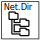
\includegraphics[width=\linewidth]{art/icons/directory2}
\end{minipage}

\section{Game}

\missionrule{Initiative Roll.}  A standard Initiative Roll determines
Initiative and Deployment, except the Initiative Roll may be made
against either your Lieutenant or your Special Agent.  In addition, in
the quadrant missions:

\begin{squishitemize}
\item The player that chose the mission receives a +3 MOD.

\item Players whose alliance controls the associated Breach Point or
  the quadrant itself get a~+3 MOD.
\end{squishitemize}

In the \textit{Datacenter} mission, teams may roll against any of
their Lieutenants and Special Agents, and the alliance which controls
more quadrants receives a~+3 MOD to the Initiative Roll.

\missionrule{Reduced Combat Groups.}  Strategic Use of Command Tokens
to nullify Orders from the opponent's Order Pool is prohibited in the
RECON+ matches.

\missionrule{Endgame.}  All matches end after three game turns.
\emph{Retreat!} rules apply as given in the main \emph{Infinity}
rulebook except the game does not end once one player has no models in
play: The remaining player may play out the game turns attempting to
score objectives.  Players do NOT automatically receive maximum points
for eliminating their opponent.

\missionrule{Destroyed.} Models are considered destroyed when they
enter the Dead state, are in a Null state at the end of the game, or
have not been deployed by the end of the game.  Those models not
destroyed are considered to have survived, as are models in
\emph{Retreat!} which evacuate the play area.

\vfill
\vbox to 0pt{}
